\chapter{Methodology}
\section{Retrieving the data}
I can access the active eBay listings near me by fetching data recursively from the eBay API. I wrote a small seeder script that stores the data in csv format and saves it locally. From there, I can easily read the csv in my notebook. The Foursquare data will be loaded within the code cells.
\section{Handling missing information and combining the two datasets}
After fetching the data, it is time to combine and unify the datasets, so I can work with coherent data in the next steps. For my purposes, it will be sufficient to have the following columns for both datasets:
\begin{itemize}
	\item Name of business/seller/store/item
	\item City
	\item State
	\item Latitude
	\item Longitude
	\item Source (eBay/Foursquare)
\end{itemize}
This is what the two datasets look like after fetching:
\begin{figure}[H]
	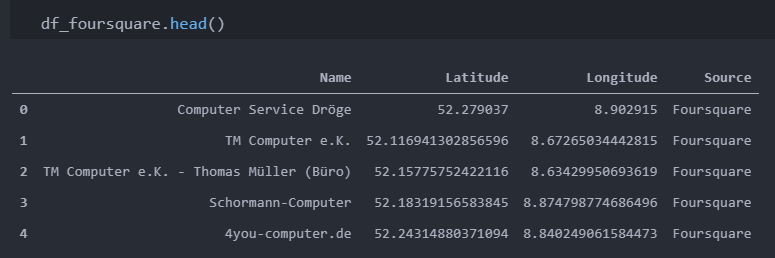
\includegraphics[width=\textwidth]{Bilder/Foursquare.PNG}
	\caption{Foursquare dataset right afer fetching with some columns already removed}
\end{figure}
\begin{figure}[H]
	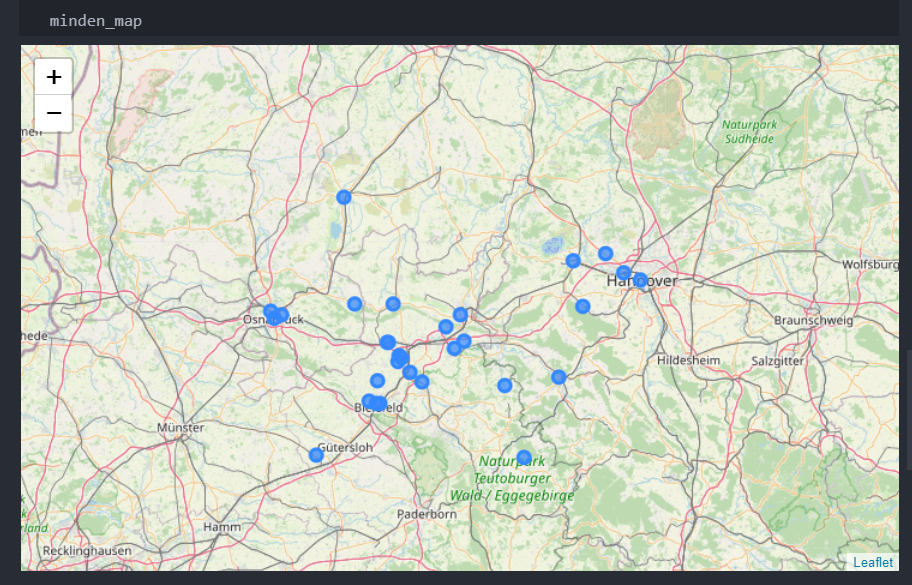
\includegraphics[width=\textwidth]{Bilder/Foursquare_Map.PNG}
	\caption{Foursquare dataset visualized in map}
\end{figure}
\begin{figure}[H]
	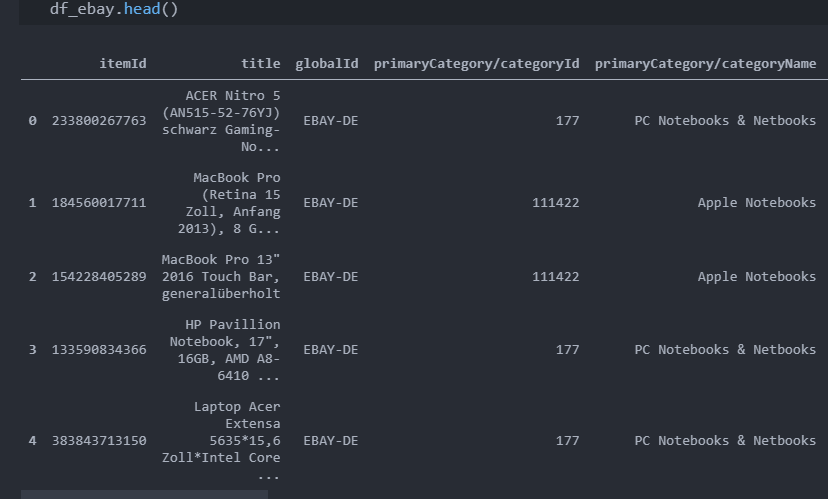
\includegraphics[width=\textwidth]{Bilder/eBay.PNG}
	\caption{Excerpt of eBay dataset right afer fetching}
\end{figure}

The Foursquare dataset is missing city and state, while the eBay dataset is missing coordinates unfortunately, as well as state. In the next step, I will preprocess the data and add the missing columns.

To preprocess the data, I will use OpenStreetMap\footnote{https://geocoder.readthedocs.io/providers/OpenStreetMap.html}. It provides a reverse geocoding function, allowing to search for locations for example by name or coordinates and receiving vast information in return. See below for the code and result.

\begin{figure}[H]
	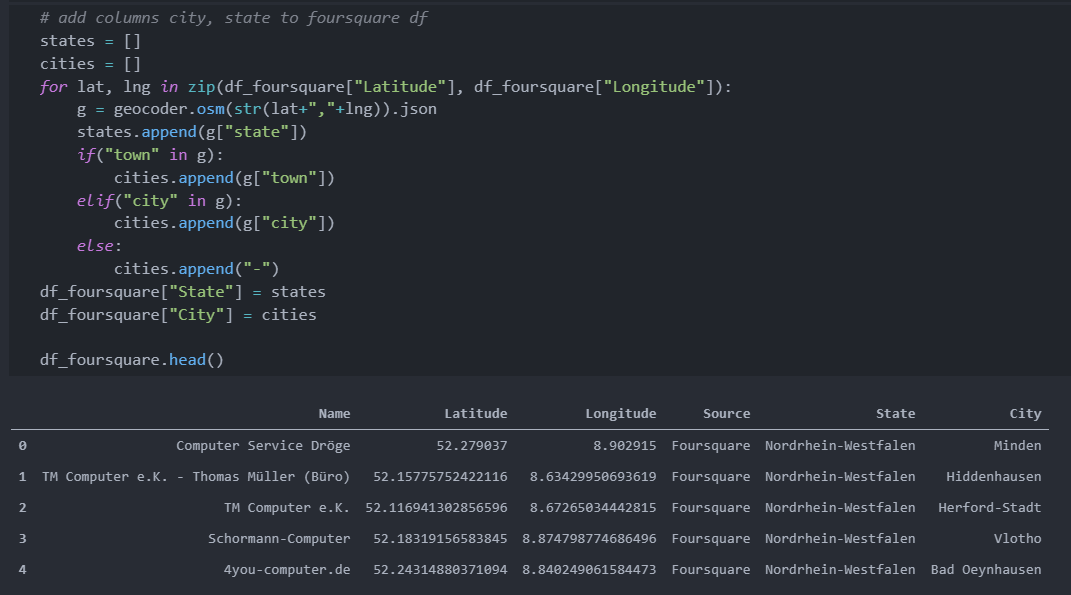
\includegraphics[width=\textwidth]{Bilder/Foursquare_preprocessed.PNG}
	\caption{Foursquare data with added state and city}
\end{figure}

The eBay data is missing state, latitude and longitude. These columns will also be added by using OpenStreetMap. See the following results.

\begin{figure}[H]
	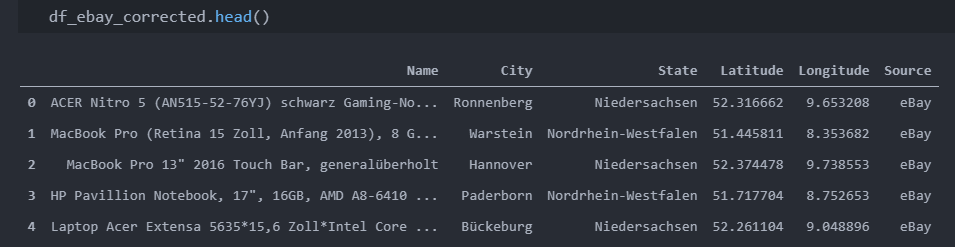
\includegraphics[width=\textwidth]{Bilder/eBay_preprocessed.PNG}
	\caption{eBay data with added state and coordinates}
\end{figure}
\begin{figure}[H]
	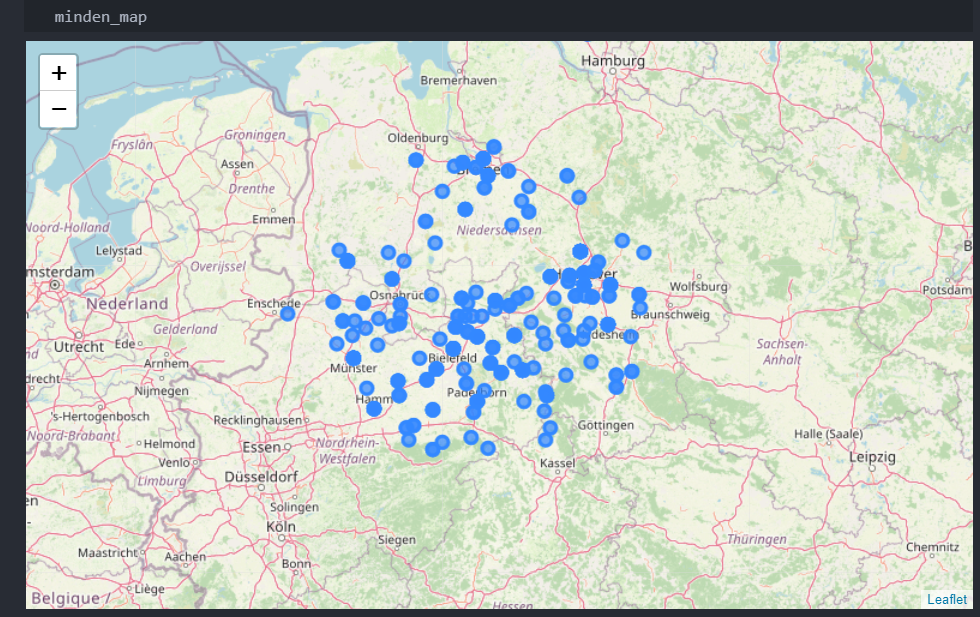
\includegraphics[width=\textwidth]{Bilder/eBay_Map.PNG}
	\caption{eBay dataset visualized in map}
\end{figure}

The two datasets are now combined and stored as a csv locally, to make sharing the data easier. This coherent structure now allows for some exploratory data analysis in the following subsections.
\section{Exploratory data analysis}
In this section, I will demonstrate how I managed to get a general overview over the data. This chapter only covers methodology, the results are discussed in \ref{results}.
\subsection{Statistical key figures and indicators}
To begin with some basic operations after creating a combined dataset, I described the given dataframe.
\begin{figure}[H]
	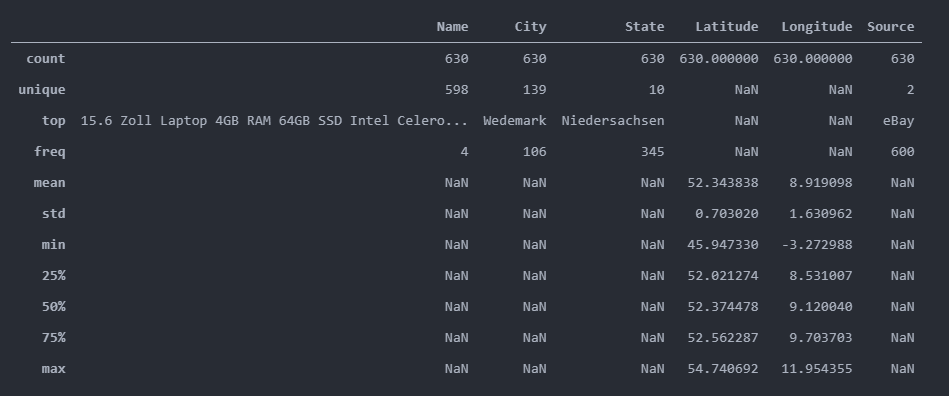
\includegraphics[width=\textwidth]{Bilder/general_findings.PNG}
	\caption{Description of dataset}
\end{figure}
\subsection{Visualizing entries using a map}
\begin{figure}[H]
	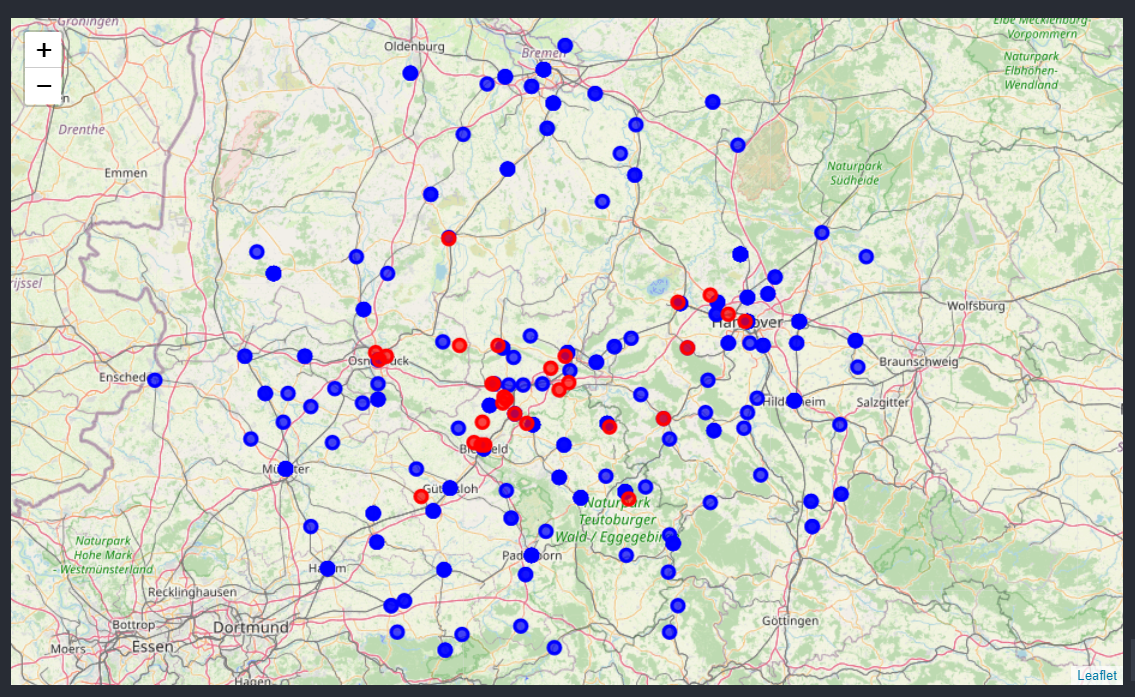
\includegraphics[width=\textwidth]{Bilder/combined_map.PNG}
	\caption{Visualization of dataset}
\end{figure}
This is what the map looks like when both sources are considered. Foursquare entries are colored red, eBay ones are blue.
\section{Inferential statistical testing}
\subsection{Similarity between data sources}
\section{Machine learning}
\subsection{Clustering entries}